% To je predloga za poročila o domačih nalogah pri predmetih, katerih
% nosilec je Blaž Zupan. Seveda lahko tudi dodaš kakšen nov, zanimiv
% in uporaben element, ki ga v tej predlogi (še) ni. Več o LaTeX-u izveš na
% spletu, na primer na http://tobi.oetiker.ch/lshort/lshort.pdf.
%
% To predlogo lahko spremeniš v PDF dokument s pomočjo programa
% pdflatex, ki je del standardne instalacije LaTeX programov.

\documentclass[a4paper,11pt]{article}
\usepackage{a4wide}
\usepackage{fullpage}
\usepackage[utf8x]{inputenc}
\usepackage[slovene]{babel}
\selectlanguage{slovene}
\usepackage[toc,page]{appendix}
\usepackage[pdftex]{graphicx} % za slike
\usepackage{setspace}
\usepackage{color}
\definecolor{light-gray}{gray}{0.95}
\usepackage{listings} % za vključevanje kode
\usepackage{hyperref}
\usepackage{titlesec}

\renewcommand{\baselinestretch}{1.2} % za boljšo berljivost večji razmak
\renewcommand{\appendixpagename}{\normalfont\Large\bfseries{Priloge}}


\titleformat{name=\section}[runin]
  {\normalfont\bfseries}{}{0em}{}
\titleformat{name=\subsection}[runin]
  {\normalfont\bfseries}{}{0em}{}


% header
\makeatletter
\def\@maketitle{%
  \noindent
  \begin{minipage}{2in}
  \@author
  \end{minipage}
  \hfill
  \begin{minipage}{1.2in}
  \textbf{\@title}
  \end{minipage}
  \hfill
  \begin{minipage}{1.2in}
  \@date
  \end{minipage}
  \par
  \vskip 1.5em}
\makeatother


\lstset{ % nastavitve za izpis kode, sem lahko tudi kaj dodaš/spremeniš
language=Python,
basicstyle=\footnotesize,
basicstyle=\ttfamily\footnotesize\setstretch{1},
backgroundcolor=\color{light-gray},
}


% Naloga
\title{Naloga 1}
% Ime Priimek (vpisna)
\author{Jakob Maležič (63170191)}
\date{\today}

\begin{document}

\maketitle

\section{Uvod.}
Pri tej nalogi smo analizirali glasovanje za Pesem Evrovizije. Predstavniki posameznih držav naj bi glasovali pristransko in pri tem favorizirali nastopajoče iz bližnjih ali sorodnih držav. Cilj naloge je bil, preveriti ali to drži.

\subsection{Podatki.}
Podatki o glasovanju za Pesem Evrovizije so bili podani v obliki csv datoteke. V datoteki je bilo zapisanih okol 33 tisoč vrstic. Vsaka vrstica je vsebovala leto glasovanja, tip glasovanja, katera država je glasovala, za katero državo je glasovala ter koliko točk ji je podelila. Točke posameznega glasovanje so se gibala med 1 in 12. Ker je bil razpon let med 1975 do 2019, se so se nekatere države večkrat pojavile kot druge, nekatere kot npr. Jugoslavija pa se po določenem letu sploh niso več.

\section{Luščenje profilov glasovanj.}
Datoteko s podatki sem prebral dvakrat. Ko sem prvič šel čez vse vrstice, sem določil vse atribute oz. stolpce. Vsak stolpec je predstavljal svoje leto glasovanja, tip glasovanja ter državo za katero je bilo glasovano. Tako sem dobil čez tisoč različnih atributov, po katerih sem profile kasneje primerjal. Ko sem drugič bral datoteko, sem za vsako državo naredil slovar, ki je vseboval prej omenjene atribute, ter vnesel vrednosti le teh. Tako pripravljen slovar, sem nato uporabil pri gručenju.

\section{Gručenje.}
Gručenje je postopek razvrščanja profilov, v našem primeru profilov glasovanj, v skupine podobnih profilov. Sestavljen je iz: računanja razdalje, ki predstavlja podobnost dveh profilov, računanja razdalje med gručami profilov, iskanjem najkrajših razdalj med gručami profilov ter združevanje le teh.

\subsection{Računanje razdalje med profili.}
Računanje razdalje med profili predstavlja največjo oviro pri gručenju. Razdaljo sem računal po evklidskem izreku. Problem se pojavi, ko profili nimajo vseh atributov. To sem rešil tako, da po takih atributih preprosto nisem primerjal in na koncu normaliziral. Če se je zgodilo da profila nista imela nobenih skupnih atributov, sem vrnil vrednost -1, da sem pri računanju razdalje med gručami vedel da le te razdalje ne smem upoštevati.

\begin{lstlisting}
# r1 ter r2 sta imeni drzav
def row_distance(self, r1, r2):

    row1 = self.data[r1]
    row2 = self.data[r2]

    sum_of_attributes = 0
    attributes_counter = 0
    for i in range(0, len(row1)):
        val1 = row1[i]
        val2 = row2[i]
        # tu preverimo ce atribut obstaja pri obeh profilih
        if val1 is not None and val2 is not None:
            sum_of_attributes += pow(val1 - val2, 2)
            attributes_counter += 1

    if attributes_counter == 0:
        return -1
    # normalizacija
    return math.sqrt((sum_of_attributes / attributes_counter) * len(row1))
\end{lstlisting}

\subsection{Računanje razdalje med gručami.}
Razdaljo med gručami sem računal z uporabo metode "Average Linkage", ki izračuna povprečno razdaljo med dvema gručama. To naredi tako, da izračuna razdalje med vsemi profili v obeh gručah in jih povpreči. Kot že prej napisano, če je bila razdalja med profiloma -1, je pri povprečenju nisem upošteval.

\subsection{Iskanje najpodobnejših gruč}
Iskanje najkrajše razdalje med dvema gručama je sedaj preprosto. Izračunati sem mogel zgolj razdalje med vsemi možnimi kombinacijami gruč ter ugotoviti katera je najkrajša.

\subsection{Združevanje v gruče.}
Gruče je sedaj enostavno zgraditi. Potrebna je zgolj ena while zanka, ki išče najpodobnejše gruče in jih združuje dokler nam ne ostane ena sama gruča.

\section{Dendrogram.}
Naloga je zahtevala tudi izris dendrograma. Na dendrogramu lahko vidimo razdalje med posameznimi profili in jih lahko tudi sami poskusimo gručiti.

\begin{figure}[htbp]
\begin{center}
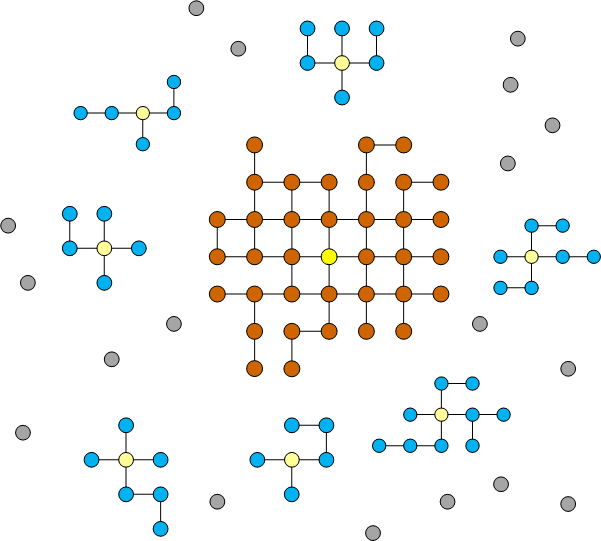
\includegraphics[scale=0.3]{slika-primer.png}
\caption{Vsako sliko opremi s podnapisom, ki pove, kaj slika prikazuje.}
\label{slika1}
\end{center}
\end{figure}


\section{Rezultati.}

V tem poglavju podaš rezultate s kratkim (enoodstavčnim)
komentarjem. Rezultate lahko prikažeš tudi v tabeli (primer je
tabela~\ref{tab1}).

Odstavke pri pisanju poročila v LaTeX-u ločiš tako, da pred novim
odstavkom pustiš prazno vrstico. Tudi, če pišeš poročilo v kakšnem
drugem urejevalniku, morajo odstavki biti vidno ločeni. To narediš z
zamikanjem ali pa z dodatnim presledkom.

\begin{table}[htbp]
\caption{Atributi in njihove zaloge vrednosti.}
\label{tab1}
\begin{center}
\begin{tabular}{llp{3cm}}
\hline
ime spremenljivke & definicijsko območje & opis \\
\hline
cena & [0, 500] & cena izdelka v EUR\\
teža & [1, 1000] & teža izdelka v dag \\
kakovost & [slaba|srednja|dobra] & kakovost izdelka \\
\hline
\end{tabular}
\end{center}
\end{table}

Podajanje rezultati naj bo primerno strukturirano. Če ima naloga več
podnalog, uporabi podpoglavja. Če bi želel poročati o rezultatih
izčrpno in pri tem uporabiti vrsto tabel ali grafov, razmisli o
varianti, kjer v tem poglavju prikažeš in komentiraš samo glavne
rezultate, kakšne manj zanimive detajle pa vključite v prilogo (glej
prilogi~\ref{app-res} in~\ref{app-code}).

\section{Izjava o izdelavi domače naloge.}
Domačo nalogo in pripadajoče programe sem izdelal sam.

\appendix
\appendixpage
\section{\label{app-res}Podrobni rezultati poskusov.}

Če je rezultatov v smislu tabel ali pa grafov v nalogi mnogo,
predstavi v osnovnem besedilu samo glavne, podroben prikaz
rezultatov pa lahko predstaviš v prilogi. V glavnem besedilu ne
pozabi navesti, da so podrobni rezultati podani v prilogi.

\section{\label{app-code}Programska koda.}

Za domače naloge bo tipično potrebno kaj sprogramirati. Če ne bo od
vas zahtevano, da kodo oddate posebej, to vključite v prilogo. Čisto
za okus sem tu postavil nekaj kode, ki uporablja Orange
(\url{http://www.biolab.si/orange}) in razvrščanje v skupine.


\begin{lstlisting}
import random
import Orange

data_names = ["iris", "housing", "vehicle"]
data_sets = [Orange.data.Table(name) for name in data_names]

print "%10s %3s %3s %3s" % ("", "Rnd", "Div", "HC")
for data, name in zip(data_sets, data_names):
    random.seed(42)
    km_random = Orange.clustering.kmeans.Clustering(data, centroids = 3)
    km_diversity = Orange.clustering.kmeans.Clustering(data, centroids = 3,
        initialization=Orange.clustering.kmeans.init_diversity)
    km_hc = Orange.clustering.kmeans.Clustering(data, centroids = 3,
        initialization=Orange.clustering.kmeans.init_hclustering(n=100))
    print "%10s %3d %3d %3d" % (name, km_random.iteration, \
    km_diversity.iteration, km_hc.iteration)
\end{lstlisting}

\end{document}